\chapter{Experiment Design}

This chapter defines how the desired outcomes defined in the Methodology chapter will practically be met. This requires describing the available code and data, how it will integrate with new code developed in this project and what the new code being developed is.

This chapter also details how the existing work in iArsenic is utilized.

\section{Well Data in iArsenic}

The data used by iArsenic can be found in the CSV in the data/ directory of iArsenic (note that this does not include CSV files in sub-directories of the data/ directory). These files have been selected on the following criteria for aggregating:

\begin{itemize}
    \item two CSV files do not include the same datapoint
    \item the CSV contains standard features required by the iArsenic models
\end{itemize}

Before preprocessing, these files contain 1,144,586 rows (including headers) combined.

The primary preprocessing function provided by iArsenic is applying name corrections. This is the process of changing region names such that a region with inconsistent naming in source data files, has the same name in an aggregate dataset. These corrections allow the well data and the geodata to be aggregated.

After preprocessing, the iArsenic data contains 868,678 rows (excluding headers). 475,182 data points are negative (safe/equal to or below 10µg/l), and 393,496 are positive (polluted / above 10µg/l), the null positive rate (the accuracy when always predicting false) is 55\%. The name corrected dataset output by iArsenic will be referred to as the iArsenic Standard Dataset.

See figure \ref{fig:x avg_datapoints} on page \pageref{fig:x avg_datapoints} for a choropleth of datapoints per District.

For a more detailed summary of the data, see table \ref{tbl:x reg_size_dp} on page \pageref{tbl:x reg_size_dp} to see the region sizes and datapoints per region.

\begin{figure}[!htb]
    \centering
    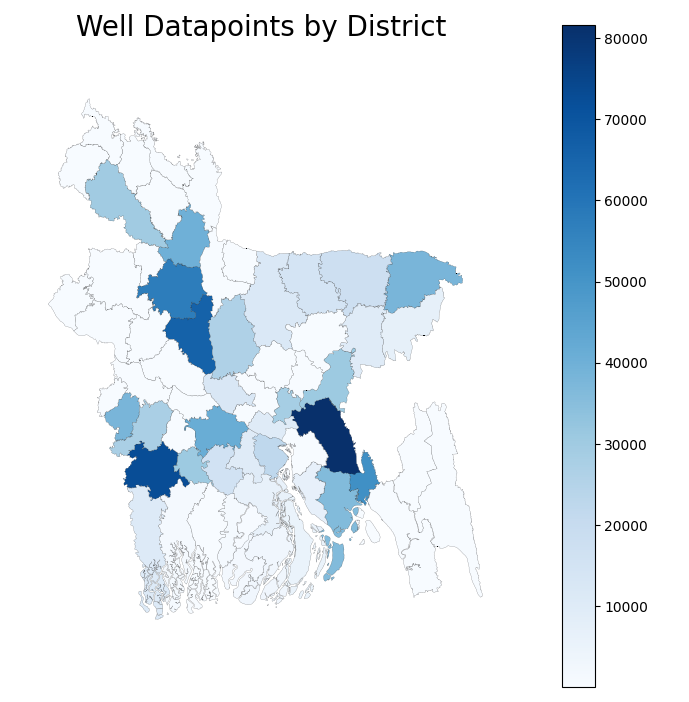
\includegraphics[scale=0.57]{figures/data_distribution_by_district.png} 
    \caption{Distribution of Well Data by District in iArsenic Standard Dataset}
    \label{fig:x avg_datapoints}
\end{figure}

\newpage

The attributes included in the iArsenic standard dataset file are the following:

\begin{itemize}
    \item Division
    \item District
    \item Upazila
    \item Union
    \item Mouza
    \item Depth
    \item Arsenic
\end{itemize}

Excluding Depth and Arsenic, attributes are region names with corresponding geographic data.

See figure \ref{fig:x labelled_divisions} on page \pageref{fig:x labelled_divisions} for a labelled map of Bangladesh divisions.

\begin{table}
    \centering
    \begin{tabular}{c c c c c c} 
         \toprule
         Name & Mean Area $km\textsuperscript{2}$ & Area $\sigma$ & Mean Data & Data $\sigma$ & Unique Values \\ 
         \midrule 
         Division & 17,482 & 6,928 & 108,584 & 72,085 & 8 \\ 
         District & 2,185 & 1,080 & 13,788 & 20,102 & 63 \\
         Upazila & 257 & 185 & 1,952 & 5,683 & 445 \\
         Union & 27 & 41 & 306 & 786 & 2,838 \\
         Mouza & 2.4 & 8.4 & 90 & 191 & 9,550 \\
         \bottomrule
    \end{tabular}
    \caption{Region sizes, datapoints per region \& count}
    \label{tbl:x reg_size_dp}
\end{table}

\begin{figure}
    \centering
    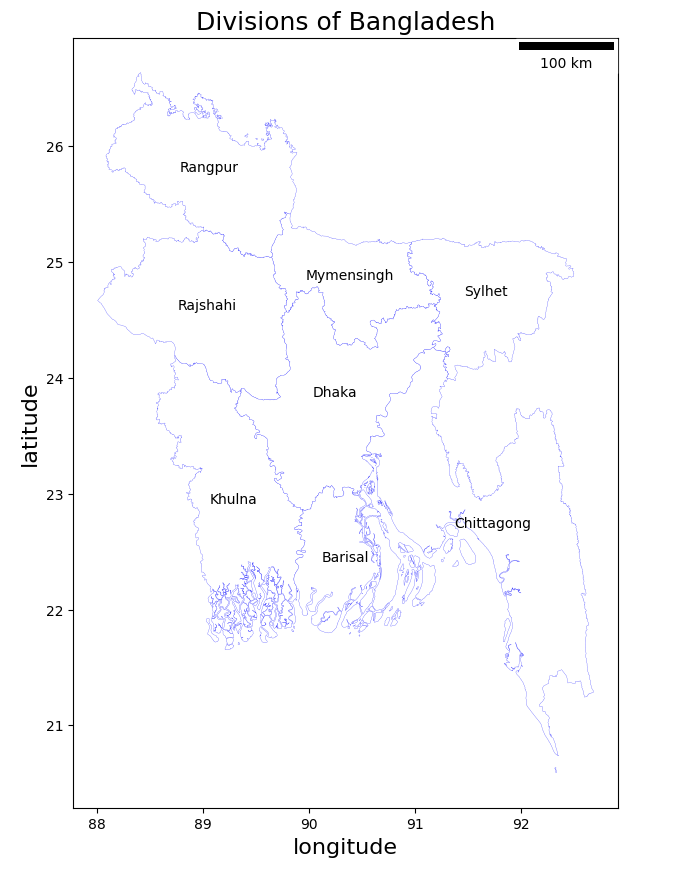
\includegraphics[scale=0.45]{figures/labelled_divisions.png} 
    \caption{The Divisions of Bangladesh mapped and labelled}
    \label{fig:x labelled_divisions}
\end{figure}

\textbf{Depth}

The Depth column refers to the depth of a well in meters.

The deepest well in the dataset is 445 meters, the lowest is 0, the is mean 40 meters and the standard deviation is 52 meters. See figure \ref{fig:x avg_depth} on page \pageref{fig:x avg_depth} for a choropleth of mean depth per Upazila and \ref{fig:x dva} on page \pageref{fig:x dva} so see the relationship between mean depth and mean arsenic by division.

\begin{figure}[!htb]
    \centering
    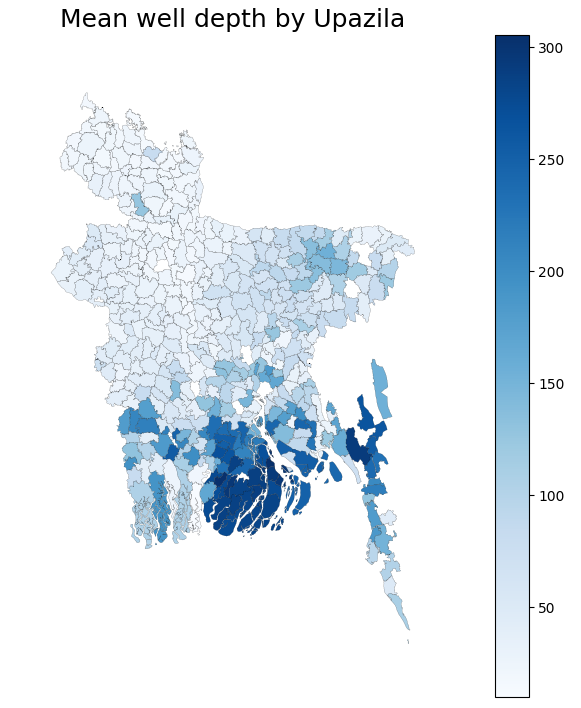
\includegraphics[scale=0.54]{figures/mean_well_depth_by_upa.png} 
    \caption{Average (mean) Well Depth by Upazila}
    \label{fig:x avg_depth}
\end{figure}

\begin{figure}[!htb]
    \centering
    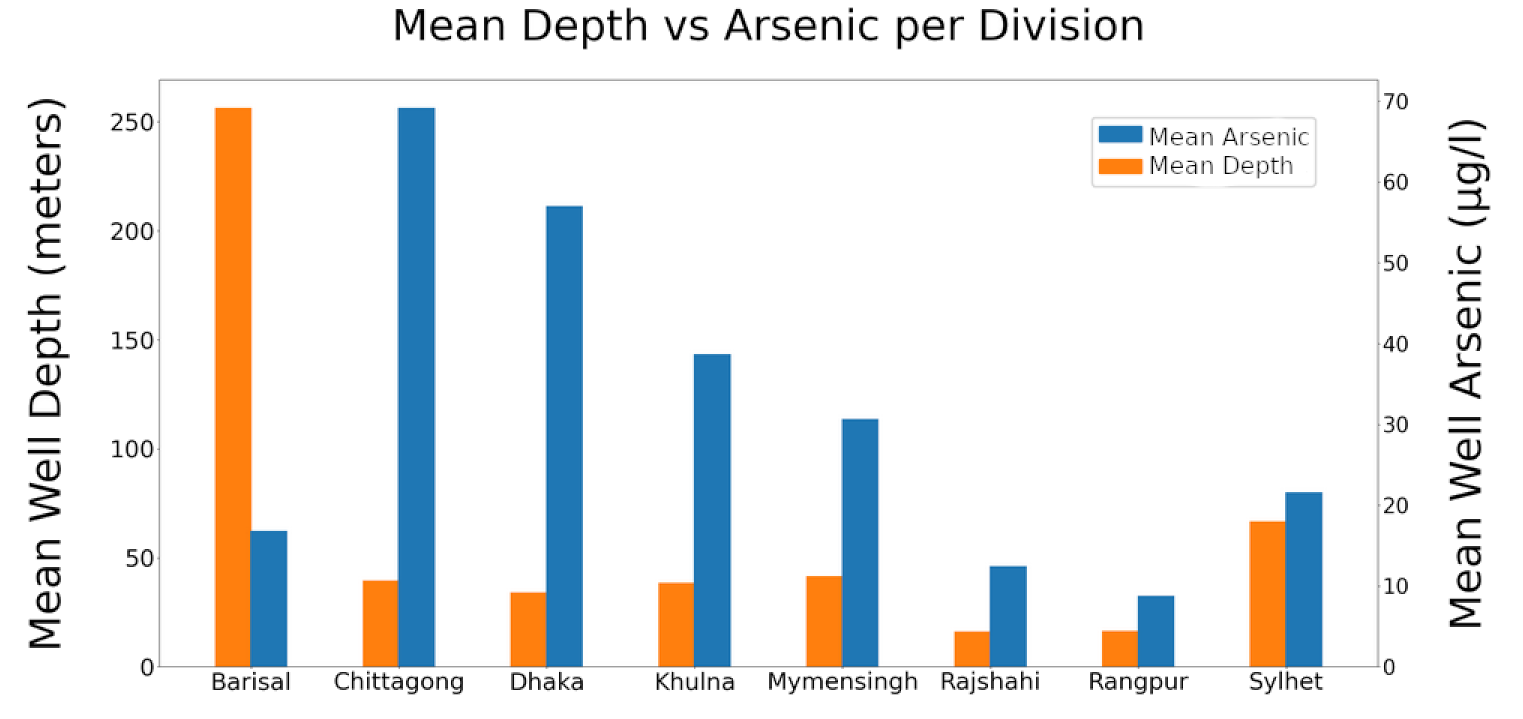
\includegraphics[scale=0.28]{figures/mean_as_vs_depth.png} 
    \caption{Chart showing the relationship between mean well depth and arsenic pollution}
    \label{fig:x dva}
\end{figure}

\textbf{Arsenic}

The Arsenic column refers to the arsenic concentration in water from a well datapoint in micro-grams per litre ($\mu$g/l).

The highest concentration of arsenic in the iArsenic standard dataset is 4,000$\mu$g/l (4ng/l), the lowest concentration of arsenic is 0$\mu$g/l, the mean is 41$\mu$g/l and the standard deviation is 74$\mu$g/l. See figure \ref{fig:x avg_as} on page \pageref{fig:x avg_as} for a choropleth of mean depth per Upazila.

\begin{figure}[!htb]
    \centering
    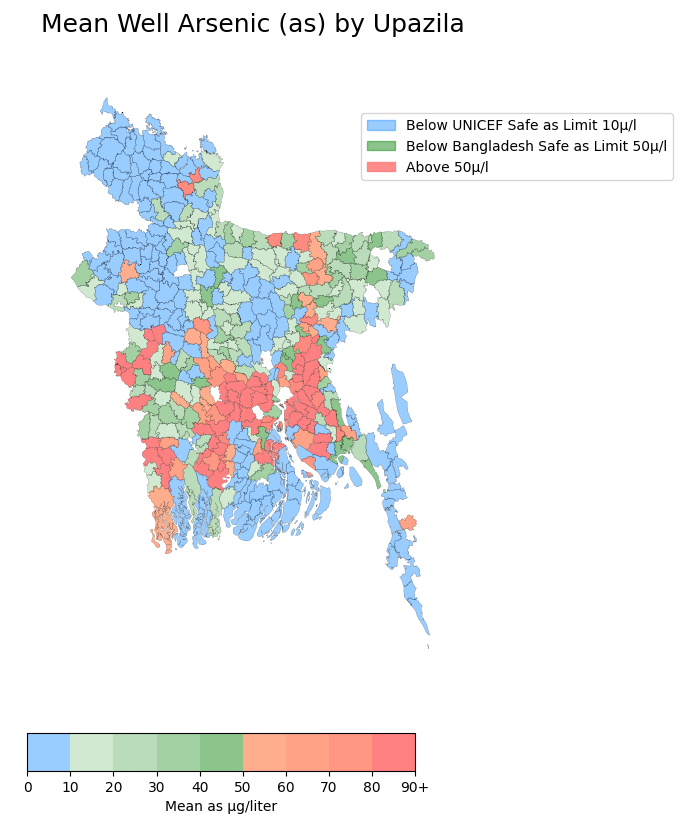
\includegraphics[scale=0.6]{figures/mean_as_by_upazila.png} 
    \caption{Distribution of Average (mean) Arsenic by Upazila in the iArsenic Standard Dataset}
    \small{See page \pageref{fig:x avg_as_cblind} for a red-green colorblind compatible version of this diagram}
    \label{fig:x avg_as}
\end{figure}

\newpage

\textbf{Why use this Dataset?}

While new and existing iArsenic models could be trained on different data, the time and resources required to produce a dataset of this quality and suitability are substantial and outside the scope of this project. 

\subsection{Geodata}

The original source of the geodata is unclear, though similar country-based polygon data can be found on the first page of Google.

The geodata has been zipped and added to the project's repository using Git Large File Storage. This is because some of the geodata are omitted from the original iArsenic repository due to it exceeding the GitHub file size limit. 

Instructions are provided in iArsenic for regenerating this missing data at the following url: \url{https://github.com/portsoc/iArsenic/tree/master/preprocessing/geodata}

\section{iArsenic Integration}

\subsection{Data Preparation}
\label{sub: data_prep}

The iArsenic code repository is downloaded from GitHub via Node Package Manager (npm). This repository includes selected source data and several tools to process this data.

Data is extracted from iArsenic using the csv-to-json.js script. This script aggregates the source files into a single data structure and outputs it as a JSON file. Additionally, it ensures that all regions follow the same naming convention, which is essential because it prevents distinct data points in the same region from appearing to be in two different regions. This enables the data to be matched to its corresponding polygon in the geodata.

The JSON file is then converted to a pandas DataFrame in Python, shuffled to ensure there is no ordering bias, and converted into 5 separate CSV files. It is split into 5 to enable k-fold cross-validation on the dataset.

These 5 CSV files are what we use to test and train the models.

See the script that generates the 5 data subsets here: \url{https://github.com/JavaRip/UoP-SoftEng-Dissertation/blob/main/utils/src_to_test_train.py}

\subsection{Generating the iArsenic Models}

iArsenic can generate 3 separate models: model3, model4 and model5.

Originally an iArsenic model was generated on all available data and then made available on the iArsenic web application. Due to their modular design, however, the models can also be imported into NodeJS.

To evaluate the models using k-folds cross-validation, each of the 3 models is generated 5 times with 4 of the CSVs used for training and 1 for testing, thus implementing k-folds cross-validation. This requires generating a total of 15 iArsenic models.

\subsection{Interfacing With Generated iArsenic Models}

Predictions are generated from the generated model using a NodeJS script. This will be referred to as the iArsenic Model Wrapper.

The predictions are saved to a temporary CSV file and the name of this file is logged to the standard output.

The iArsenic model wrapper requires the following parameters to be passed as system arguments:
\begin{itemize}
  \item a CSV file containing the data points to use to generate predictions
  \item the stain colour of the well the data point is from
  \item the model to generate the prediction from
  \item the k-fold version of the model to generate the prediction from
\end{itemize}

Initially, the iArsenic Wrapper Script would produce an estimate from one data point at a time, passed as a system argument. However, this would take days to pass the every datapoint in the test dataset. Therefore the test dataset is passed as a CSV file path, which takes less than an hour to process.

\subsection{Imputing Stain Colour}

In the original iArsenic web application, the stain colour was to be specified by a user entering parameters about a real well, requiring the user to observe and provide the staining colour of the well. The data extracted from iArsenic however did not include staining colour data. 

When working with missing values there are primarily 3 options (see \cite{Aurélien2017} page 88): 

\begin{enumerate}
    \item remove the feature with missing values
    \item delete all rows containing missing data
    \item replace missing data with a fixed value
\end{enumerate}

Because the iArsenic models will not run with the colour omitted, option 1 is not viable. Because none of the rows contain staining data, option 2 is also not viable. Therefore we must fill in the data with a fixed value, either 'Red' or 'Black'.

To determine whether the value should be set to 'Red' or 'Black', the models have been evaluated using each and the value with which the model performs best, 'Red', has been selected. Figure \ref{fig:x ia_model_black_red_accuracy} on page \pageref{fig:x ia_model_black_red_accuracy} shows the accuracy of the iArsenic models with 'Black' or 'Red' used as the imputed well colour.

\begin{figure}[h]
    \centering
    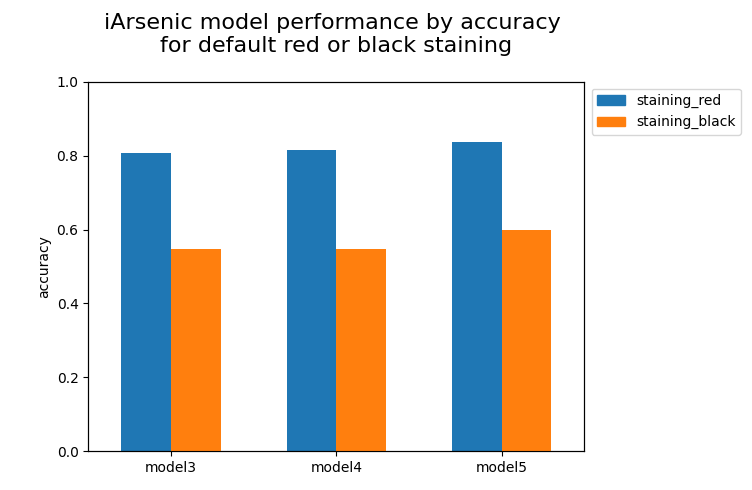
\includegraphics[scale=0.55]{figures/ia_model_black_red_accuracy.png} 
    \caption{iArsenic model performance by accuracy for default red vs black staining}
    \label{fig:x ia_model_black_red_accuracy}
\end{figure}

\newpage

Considering the accuracy score alone, it appears that setting the parameter to 'Red' produces the best model performance by approximately 20\%. As mentioned in \cite{EM} on page \pageref{EM}, a higher accuracy score however does not guarantee that one model outperforms another.

Comparing the sensitivity and specificity of the models shows that when the staining is set to 'Black' model3 and model4 always assume the well is safe. The sensitivity, the true positive rate, becomes 0 and the specificity, the true negative rate, becomes 1. While the specificity is lower when the staining is set to 'Red', the sensitivity is much higher for each model, indicating better performance. See \ref{fig:x ia_svs_red} on page \pageref{fig:x ia_svs_red} for the sensitivity and specificity plotted as a bar chart for 'Red' and 'Black staining for comparison.

\newpage

\begin{figure}[!htb]
    \centering
    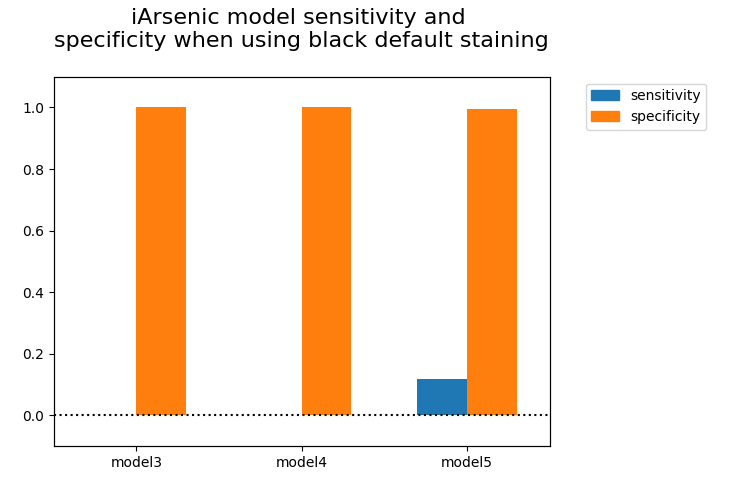
\includegraphics[scale=0.55]{figures/ia_models_sensitivity_vs_specificity_black.png} 
    \label{fig:x ia_svs_black}

    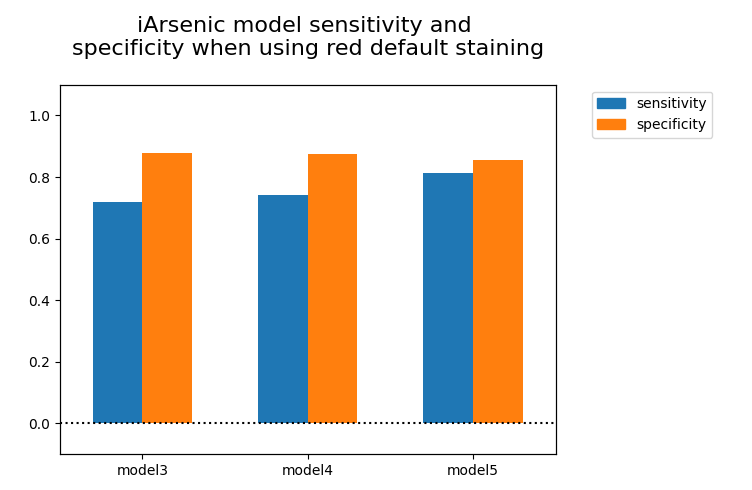
\includegraphics[scale=0.55]{figures/iarsenic_model_sensitivity_vs_specificity_red.png} 
    \caption{Model sensitivity and specificity stain parameter 'Black' (top) vs 'Red' (bottom)}
    \label{fig:x ia_svs_red}
\end{figure}

\newpage

Generating two confusion matrices for model5, one generated from 'Black' passed as a parameter and one from 'Red', reinforces the conclusion that using 'Red' as a parameter produces a better model. See \ref{fig:x Confusion Matrix mode5 Red Staining} on page \pageref{fig:x Confusion Matrix mode5 Red Staining} to see a confusion matrix for each staining parameter for comparison of evaluations.

\begin{figure}[!htb]
    \centering
    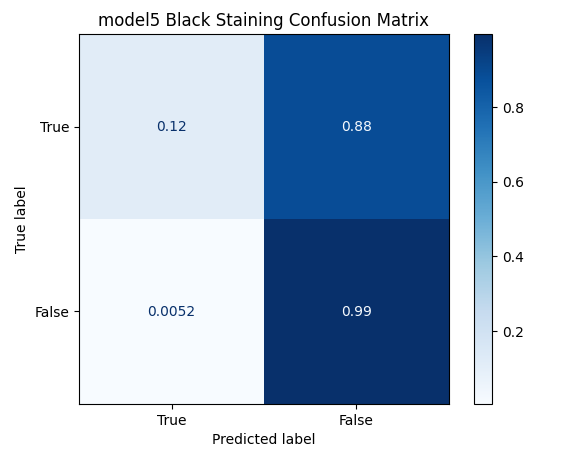
\includegraphics[scale=0.6]{figures/m5_black_cm.png} 
    \label{fig:x Confusion Matrix mode5 Black Staining}
    
    \centering
    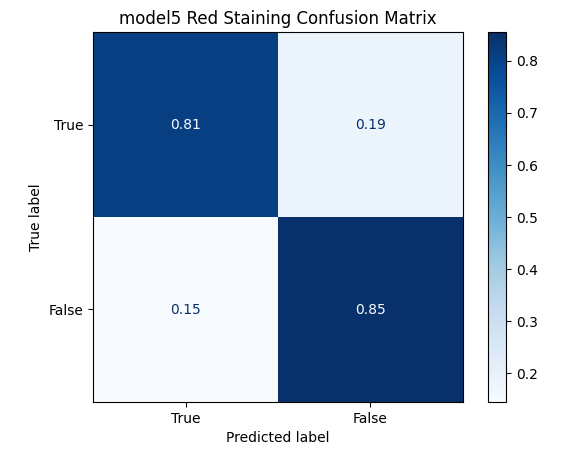
\includegraphics[scale=0.6]{figures/m5_red_cm.png} 
    \caption{Confusion Matrix model5 'Black' (top) vs 'Red' (bottom) Staining}
    \label{fig:x Confusion Matrix mode5 Red Staining}
\end{figure}

\newpage

\textbf{Quantitative Approach to Selecting Staining Parameter}

Observing the evaluation metrics of the iArsenic models and comparing them when producing predictions with either 'Red' or 'Black' as the staining parameter has indicated that the models perform better with 'Red' passed as a parameter. This is however still arguably down to interpretation.

A quantitative comparison of the models, using a value such as area under the curve would be a beneficial addition to the evaluation. This however is not possible with the iArsenic models as there is no feature to change the classification threshold, which is required to generate a receiver operating curve and therefore calculate the area under the curve.

\section{Creating a Common Model Interface}

The machine learning models will be made in Python. These can be interfaced with directly using Python modules with parameters passed directly into function calls. This is inconsistent with the iArsenic models which are run via the iArsenic Wrapper Script using node, passing parameters with command line arguments.

A Common Module Interface has therefore been specified which standardises how the modules should be interacted with. This interface specifies that each model will have a main function which takes two parameters, the test data source and the k-fold number, and returns predictions as a pandas DataFrame.

\subsection{Implementing the Common Model Interface}

Each model has a directory in the top-level models directory. Each model directory contains a model.py file which exports a Python module which can generate predictions based on the Common Module Interface, in addition to any other resources required by the model. See \ref{fig:x p_fs} on page \pageref{fig:x p_fs} for an illustration of this file structure.

Because it is a NodeJS script, the iArsenic Model Wrapper cannot accept variables passed by Python. Therefore a Python to NodeJS Bridge has been created. The Python to NodeJS Model Bridge works by running the iArsenic Model Wrapper from Python in a subprocess managed by Python from the main.py script.

\section{Evaluating the Models}

The predictions returned from the common model interface are used for evaluation. The following evaluation metrics are generated:
\begin{itemize}
  \item accuracy
  \item sensitivity 
  \item precision 
  \item specificity 
  \item f1
\end{itemize}

See \ref{EM} on page \pageref{EM} for a detailed explanation of these metrics.

\subsection{Standardizing Classifications}

The iArsenic models generate predictions from 1 of three classifications, safe, polluted, highlyPolluted. The scikit-learn models could be configured to output any number of classifications.

To adhere to conventional evaluation metrics the iArsenic predictions were simplified to safe or polluted, where highlyPolluted predictions are converted to polluted. This enables the metrics detailed in \ref{EM} on page \pageref{EM} to be used instead of defining our own evaluation methods and metrics, which would be less comparable to other real-world models.

\section{Creating a Main Script to Run \& Evaluate Experiments}

The Common Module Interface allows the models imported to the main.py script and run programmatically, without specific code defined for each model. 

This facilitates maintainable code as the complexity of the code increases. The complexity of the main.py script necessitates that steps to ensure maintainability are taken. 

Significant complexity has been introduced in making the models run and build concurrently. This is important however as doing this sequentially would take more time than is practical.

The iArsenic models benefit the most from being run concurrently as these are single-threaded. Running them concurrently allows more of the host machine's CPU power to be utilised by using multiple CPU cores simultaneously.

The machine learning models however are written using scikit-learn libraries, which are able to use all CPU cores available. 

Further optimizing the models by, for example, running the iArsenic models concurrently and the machine learning models sequentially was not deemed necessary, as building and running all models concurrently took approximately 3.5 days, which is a practical amount of time. This run was achieved on a server computer with Ubuntu 22.01, an 8 x 1.8GHz core CPU and 96GB 1600MHz DDR3 RAM.

\subsection{Main Script Structure}

The purpose of the main.py script is to provide an entry point to execute all required steps of the project.

The main script takes the following steps:
\begin{enumerate}
    \item extract the iArsenic \& geodata
    \item generate the k-folds cross-validation data split 
    \item build the iArsenic models
    \item generate predictions from all models
    \item generate an evaluation for each model's predictions
\end{enumerate}

\section{Development of New Models}

In the existing work section of the literature review \ref{ew} on page \pageref{ew}, 3 model approaches were examined.

The iArsenic models implement elements of k-nearest neighbour algorithms, \cite{Winkel2008} used random forests. This makes these model types candidates for further experimentation. Multilayer feed-forward neural network classifiers are also used because of their versatility in machine learning.

The models in both \cite{Winkel2008} and \cite{Connolly2022} ues latitude and longitude. Because of the availability of geodata in this project, preprocessing regions to their latitude and longitude is considered a viable technique. 

The iArsenic models calculate global variables during preprocessing, including the lower quartile, upper quartile and median arsenic concentrations for any given region. This processed data can be extracted from the iArsenic model and passed to a machine-learning model.

Another preprocessing technique used is applying no preprocessing.

When initially developing a model, intuition is used to hypothesize how a model might potentially work. After being implemented in code it is optimized. Neural networks have required substantial optimizations to allow the models to be trained and produce predictions within hours instead of days or weeks, at the compromise of model performance.

The predicted suitability of these model types is reinforced by \cite{Caruana2006} when comparing the performance of machine learning algorithms over different types of datasets.

\subsection{Summary of Models and Preprocessing Techniques Implemented}

\textbf{Types of Model}

\begin{enumerate}
    \item K-Nearest Neighbours Classifier
    \item Random Forest Classifier
    \item Multilayer Perceptron Feed Forward Neural Network Classifier
\end{enumerate}

\textbf{Types of Preprocessing}

\begin{enumerate}
    \item No preprocessing
    \item Conversion of region names to latitude and longitude
    \item Extracting iArsenic model preprocessed data
\end{enumerate}

\subsection{model6}

Model6 is an implementation of scikit-learn's random forest classifier with the default configuration.

Because this model cannot process string values, all string values are converted to numerical values, with each new string given an identification number in ascending order.

No preprocessing is applied to the data.

\subsection{model7}

Model7 is also a default implementation of scikit-learn's random forest classifier. This model incorporates computed region attributes computed in model5.

model5 uses feature engineering to calculate the median, lower quartile and upper quartile of the arsenic in a region, for a given depth range.

The hypothesis is that this feature engineering will provide the model with information that correlates with the model prediction target for a given data point, improving the models performance.

These values are therefore incorporated into the dataset used for model7. Where the values for a region are missing from the model5 dataset, the values from the region's parent are used.

\subsection{model8}

Model8 uses a feed-forward neural network, scikit-learn's MultiLayer Perceptron Classifier (MLPClassifier) model. See the configuration of model8 in table \ref{tbl:x m8_config} on page \pageref{tbl:x m8_config}.

\textbf{Neural Network Configuration}

\begin{table}
    \centering
    \begin{tabular}{c c c c c} 
         \toprule
         Hidden Layers & Solver & Learning Rate & Epochs & Validation \\ [0.5ex] 
         \midrule
         3 & adam & adaptive & 100 & 10\% of train\\ 
         \bottomrule
    \end{tabular}
    \caption{Model8 MLP configuration}
    \label{tbl:x m8_config}
\end{table}

The first hidden layer consists of half the number of inputs, the next hidden layer one-quarter the number of inputs and the final hidden layer one-eighth. The adam algorithm is used because it is generally faster than standard gradient descent on datasets this size. An adaptive learning rate is used to allow the performance to increase up to the maximum limit of 100 epochs.

\textbf{Data Preprocessing \& Feature Engineering}

The median, upper quartile and lower quartile arsenic values are imported from the model5 processed data to the dataset used by this model.

The smallest region size, the Mouzas are one hot encoded, allowing each Mouza to have a corresponding input node.

The region columns are dropped.

The data is normalised between 0 and 1.

\textbf{Model Optimization}

Due to the number of Mouzas (9550), the model could not allocate enough memory to run with the source data passed directly.

Therefore the source data has been split into 8 subsets by Division (See figure \ref{fig:x labelled_divisions} on page \pageref{fig:x labelled_divisions}. For each Division a model is trained with the data points within that region and predictions are generated. These predictions are then added to their corresponding data points in the source dataset.

The implementation of this optimization can be seen in figure \ref{fig:x m8_code} on page \pageref{fig:x m8_code}.

\begin{figure}[h]
    \begin{minted}[linenos]{python3}
  for div in train_df['Division'].unique():
    tr_div = train[train['Division'] == div]
    te_div = test[test['Division'] == div]
    
    tt_df = append_test_train(te_div, tr_div)
    
    conv_cat_num(tt_df, 'Label')
    tt_df = ohe_col(tt_df, ['Mouza'])
    
    tt_df = tt_df.drop(
      columns=[
        'Division',
        'District',
        'Union',
        'Upazila',
      ]
    )
    
    cat_int_enc(tt_df)
    tt_df = pd.DataFrame(
      MinMaxScaler().fit_transform(tt_df), 
      columns=tt_df.columns
    )
    
    te_div, tr_div = split_test_train(tt_df)
    
    train_X = tr_div.drop(['Arsenic', 'Label'], axis='columns')
    train_y = tr_div['Label']
    test_X = te_div.drop(['Arsenic', 'Label'], axis='columns')
    
    num_feat = len(test_X.columns)
    
    clf = MLPClassifier(
      solver='adam',
      alpha=0.0001,t
      hidden_layer_sizes=(
        math.trunc(num_feat / 2), 
        math.trunc(num_feat / 4), 
        math.trunc(num_feat / 8)
      ),
      learning_rate='adaptive',
      random_state=99,
      max_iter=100,
    )
    
    clf.fit(train_X, train_y)
    
    test.loc[test['Division'] == div, ['Prediction']] = clf.predict(test_X)
    \end{minted}
    \caption{Snippet showing m8 optimization method, where a different model is trained for each of the 8 Divisions}
    \label{fig:x m8_code}
\end{figure}

\subsection{model9}

model9 is also based on scikit-learn's MLPClassifier. See the configuration of model9 in table \ref{tbl:x m9_config} on page \pageref{tbl:x m9_config}.

\textbf{Neural Network Configuration}

\begin{table}
    \centering
    \begin{tabular}{c c c c c} 
         \toprule
         Hidden Layers & Solver & Learning Rate & Epochs & Validation \\ [0.5ex] 
         \midrule
         2 & adam & adaptive & 100 & 10\% of train\\ 
         \bottomrule
    \end{tabular}
    \caption{Model9 MLP configuration}
    \label{tbl:x m9_config}
\end{table}

The first hidden layer consists of 50 nodes, the next hidden layer consists of 2 nodes. An adaptive learning rate is used to allow the performance to increase up to the maximum limit of 100 epochs.

\textbf{Data Preprocessing \& Feature Engineering}

The source data is merged with the geodata and each datapoint is attributed with a latitude and longitude. All other feature columns are dropped.

Simplifying the dataset to just latitude and longitude enables the entire dataset to be used to train and test the model.

\subsection{model10}

model10 uses scikit-learn's of the k-nearest neighbours classification algorithm, the KNeighborsClassifier. The number of neighbours is set to 50.

\textbf{Data Preprocessing \& Feature Engineering}

The source data is merged with the geodata and the latitude and longitude of each Mouza is attributed to each datapoint. All other feature columns are dropped.

This model will find the 50 data points with the smallest difference in terms of latitude, longitude and depth in the training set then make a prediction from the classification of these data points.

\subsection{model11}

Like model10, model11 uses scikit-learn's implementation of the k-nearest neighbours classification algorithm. The number of neighbours is set to 250.

\textbf{Data Preprocessing \& Feature Engineering}

This model uses the data processed by model5, including the lower median and upper quartile arsenic values for a region.

This model will find the 250 data points with the smallest difference in the median, lower quartile and upper quartile values of arsenic in the training dataset and make a prediction from the most common classification of those nearby data points.

\subsection{model12}

Model12, an ensemble model, uses prediction data from all models to identify which model performs best in which region.

For any data point, the model which performs best in this region could be used to generate the predictions, utilising the best of all models.

As of the date of submission, model12 is a work in progress because of limitations of the common model interface, this will be detailed further in the Future Work chapter.

A file showing which model performed best for each k-fold can be seen here: \url{https://github.com/JavaRip/UoP-SoftEng-Dissertation/blob/main/models/model12/best_model_by_upa.csv}

\subsection{model13}

Like model10 and model11, model13 uses scikit-learn's k-nearest neighbours classification algorithm, the number of neighbours is set to 5000 neighbours.

Figure \ref{fig:x aod} on page \pageref{fig:x aod} shows how arsenic levels link to depth. This illustrates why categorizing a datapoint based on data points in another depth category will indicate a lower or higher arsenic concentration.

\begin{figure}[!htb]
    \centering
    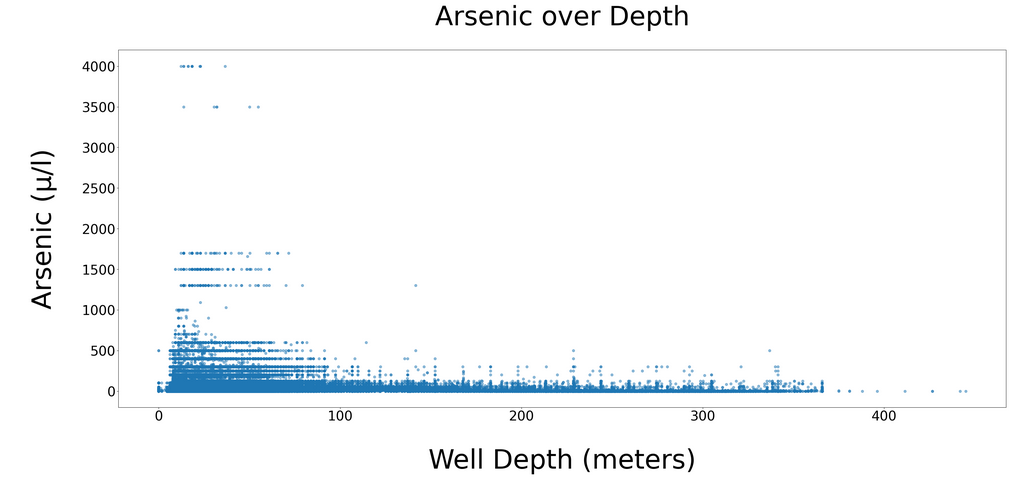
\includegraphics[scale=0.43]{figures/arsenic_over_depth.png} 
    \caption{Distribution of Well Data by District in iArsenic Processed Dataset}
    \label{fig:x aod}
\end{figure}

\textbf{Data Preprocessing \& Feature Engineering}

Model13 trains a separate model for each depth strata. This eliminates the possibility of all nearest neighbours of a data point being from the same region at a different depth. 

Comparing a neighbouring data point at a different depth is wrong because deeper wells will almost always be safer. Therefore wells in the same depth range should be used as neighbours.

In addition to being split into separate depth categories, all features are removed apart from the latitude and longitude.

\subsection{Model14}

Like model8, model14 splits the data into smaller subsets. Instead of splitting the data by the Division, it is split by the depth category. See \ref{tbl:x m14_config} on page \pageref{tbl:x m14_config} to see the configuration of model14.

\textbf{Data Preprocessing \& Feature Engineering}

The data is reduced to the latitude and longitude of each data point. Every column apart from Depth is dropped. All columns are normalised to between 0 and 1.

\begin{table}
    \centering
    \begin{tabular}{c c c c c} 
         \toprule
         Hidden Layers & Solver & Learning Rate & Epochs & Validation \\ [0.5ex] 
         \midrule
         2 & adam & adaptive & 100 & 20\% of train\\ 
         \bottomrule
    \end{tabular}
    \caption{Model14 MLP configuration}
    \label{tbl:x m14_config}
\end{table}

\section{Conclusion}

This chapter describes the landscape in which the machine learning models have been developed by detailing the practicalities of the available data and the existing iArsenic models.

This illustrates the foundation the machine learning models have been developed upon, explaining their design with regard to the requirements and opportunities presented by the existing work.

In the next chapter, Results and Evaluation, the outcome of the experiment execution is evaluated in the context of the desired outcomes defined in the Methodology in section \ref{desired_outcomes} page \pageref{desired_outcomes}. 